
\documentclass{article} % For LaTeX2e
\usepackage{iclr2026_conference,times}

% Optional math commands from https://github.com/goodfeli/dlbook_notation.
\input{math_commands.tex}

\usepackage{hyperref}
\usepackage{url}
\usepackage{bbm}
\usepackage{subcaption}
\usepackage{graphicx}
\usepackage{amsthm}
% \usepackage{natbib}
% \usepackage{subfigure}

\title{Conformal Decision Theory for AI Agents}

\author{
    Drew Prinster \& Samuel Stanton \\
    Genentech \\
    1 DNA Way, San Francisco, CA \\
    \texttt{\{prinster.drew,stanton.samuel\}@gene.com}
}

\newcommand{\fix}{\marginpar{FIX}}
\newcommand{\new}{\marginpar{NEW}}
\newcommand{\drew}[1]{\textcolor{blue}{[Dr: #1]}}


% \iclrfinalcopy % Uncomment for camera-ready version, but NOT for submission.
\begin{document}


\maketitle

\begin{abstract}
Enabling AI agents to automate or inform high-stakes decision making inevitably involves risks, but it is often precisely in real-world, high-stakes settings where those risks are most difficult to control or quantify. Prime examples include iterative biomolecular design and active learning, where merely enabling an AI system to generate or query its next datapoint induces feedback-loop shifts in the data distribution that can cause standard uncertainty- and risk-quantification methods to deteriorate or break down entirely. This paper develops Conformal Decision Theory for AI Agents: a practical and statistically-principled methodological framework for enabling black-box AI agents to automatically determine their own ``zone of competence'' based on their available training data, to design experiments with a (marginal) guarantee on the hit rate (or on some other user-specified criteria of interest). Underlying this framework is our algorithm for ``conformal policy control,'' which generalizes prior methods for conformal risk control to both non-exchangeable data distributions and to broader risk functions. We demonstrate the utility of our methods on real-world datasets. 
\end{abstract}


\section{Outline}

\subsection{Problem sketch}

Note: Currently this is abusing the terms of ``utility'' and ``loss''---which are perhaps better understood as ``reward'' and ``cost'' in RL terminology---to refer to distinct quantities, for the sake of consistency with prior methods that we will generalize (e.g., conformal risk control \citep{angelopoulos2022conformal}), though we will rethink this in revisions.

\textbf{Notation:}
\begin{itemize}
    \item \textit{Inputs/contexts:} $\mathbf{x}\in\mathcal{X}$ \quad (e.g., possible protein sequences $\mathbf{x}\in \mathcal{V}^*$, for a vocabulary $\mathcal{V}$)
    \item \textit{Outcome/response space:} $\mathbf{y}\in\mathcal{Y}$ \quad (e.g., binding affinity)
    \item \textit{Actions:} $a:\mathcal{X}\rightarrow \mathcal{X}$ \quad (e.g., modifying a seed seq. $\mathbf{x}$ to a designed seq. $\mathbf{x}'$: $a(\mathbf{x})=\mathbf{x}')$
    \item \textit{Loss/cost:} $L_t:=l(a(\mathbf{x_t}), \mathbf{x_t}, \mathbf{y_t})$ \quad (e.g., if designed seq. not in feasible set $\mathcal{F}$: \qquad \quad $L_t=\mathbbm{1}\{\mathbf{x_t'}\not\in \mathcal{F}\}$)
    \item \textit{Utility/reward:} $U_t := u(a(\mathbf{x_t}), \mathbf{x_t}, \mathbf{y_t})$ \quad (e.g., improved binding affinity of designed seq. relative to seed: $U_t = \max((\mathbf{y_t'} - \mathbf{y_t}), 0)$)
\end{itemize}

\textbf{General ideal goal:} 
\begin{align*}
    \argmax_{a_t}\quad u(a_t(X_t)) \quad \text{s.t.} \quad L_t \leq \alpha.
\end{align*}

\textbf{General proxy problem:} For policy $p_t:=p_t(\cdot\mid \mathcal{D}_t)$,
\begin{align*}
    \argmax_{p_t}\quad \mathbb{E}_{a_t\sim p_t}[u(a_t(\mathbf{x_t}))] \quad \text{s.t.} \quad \mathbb{E}_{a_t\sim p_t}[L_t\mid L_{<t}] \leq \alpha.
\end{align*}


\textbf{Protein design proxy problem:} Setting $a_t(\mathbf{x_t}) = {\color{blue}u(\mathbf{x_t}, \mathbf{x_t'})}$ and $L_t = {\color{blue}\mathbbm{1}\{\mathbf{x_t'}\not\in \mathcal{F}\}}$, 
\begin{align*}
    \argmax_{p_t}\quad \mathbb{E}_{a_t\sim p_t}[{\color{blue}u(\mathbf{x_t}, \mathbf{x_t'})}] \quad \text{s.t.} \quad \mathbb{E}_{a_t\sim p_t}[{\color{blue}\mathbbm{1}\{\mathbf{x_t'}\not\in \mathcal{F}\}} \mid L_{<t}] \leq \alpha,
\end{align*}
where the utility is determined by improved outcomes (e.g., binding affinity) within some edit distance, subject to feasibility:
\begin{equation}
u(x, x') = \begin{cases}
\max(y' - y, 0) & \text{if } x \in \mathcal{F} \text{ and } x' \in \mathcal{F} \\
1 & \text{if } x \notin \mathcal{F} \text{ and } x' \in \mathcal{F} \\
0 & \text{if } x \notin \mathcal{F} \text{ and } x' \notin \mathcal{F} \\
-1 & \text{if } x \in \mathcal{F} \text{ and } x' \notin \mathcal{F}.
\end{cases}
\end{equation}
See Section \ref{sec:algorithm} for more details on the proposed approach---the high-level idea is to enforce the constraint using conformal risk control (CRC) \citep{angelopoulos2022conformal} extended to an \textit{online} setting under multi-step feedback covariate shift (MFCS) \citep{prinster2024conformal}.


\subsection{Sketch of key challenges \& planned technical contributions}


\begin{table}[ht]
\begin{tabular}{|p{0.3\linewidth}|p{0.34\linewidth} | p{0.34\linewidth}|}
\hline
 \textbf{Topic} & \textbf{Challenge} & \textbf{Planned contribution} \\ \hline
1. Risk control under feedback-loop shifts: &   Standard conformal risk control (CRC) \citep{angelopoulos2022conformal} is not valid under MFCS &  Extending CRC to weighted version for MFCS validity \\ \hline
2. Marginal vs. ``trajectory-conditional'' guarantee: & Limitations of marginal guarantee (i.e., risk control may not hold for particular trajectory) & \textit{Online} CRC should have stronger, ``trajectory-conditional'' guarantee (i.e., conditional on previous losses)  \\ \hline
3. Compute complexity & CP weights for MFCS in \citet{prinster2024conformal} have factorial complexity ($\mathcal{O}(t!)$) & Potential solution treating $T-1$ previous distributions as a single \textit{mixture}; results in linear time computation: $\mathcal{O}(t)$ \\ 
\hline
4. Asymptotic efficiency result (?) & Ideally could show that CDT method converges asymptotically & Seems like should be able to generalize Theorem 3 in \citet{vovk2018conformal}, as think our method is a generalization of their Algorithm 1 \\ 
\hline
5. Generative search setting: & Previous work has assumed \textit{fixed library} of possible actions/sequences. (Main challenge to doing this is how to normalize the weights.) & Should be able to treat this as an expanding library/resampled library at each timestep; just need to keep track of policy's support.  \\ \hline
\end{tabular}
\end{table}


Preliminary promising experimental results on mixture-weights approach to computing weights (planned contribution 4):

% \begin{figure}[!htb]
%     \centering
%     \includegraphics[width=0.5\textwidth]{figures/SplitCPActiveLearning_unbounded_meps_title.pdf}
%     \\
%     \hfill
%         \includegraphics[width=0.32\textwidth]{figures/SplitCPActiveLearning_unbounded_meps_coverage.pdf}
%     \hfill
%         \includegraphics[width=0.32\textwidth]{figures/SplitCPActiveLearning_unbounded_meps_width.pdf}
%     \hfill
%         \includegraphics[width=0.32\textwidth]{figures/SplitCPActiveLearning_unbounded_meps_MSE.pdf}
%     \hfill
%     \\
% % \caption{

% %     }
% \label{fig:SplitCP_ActiveLearningExpts}
% \end{figure}


\subsection{Comparison to of proposed CDT guarantees to conformal prediction and conformal risk control}

Note: In all the following, $\lambda$ controls the ``conservativeness,'' with the risk non-increasing in $\lambda$:

\textbf{Conformal prediction} \citep{vovk2005algorithmic} (miscoverage) guarantee:
\begin{align*}
    \mathbb{E}\Big[\mathbbm{1}\big\{Y_t\not\in \widehat{C}_{\lambda}(X_t)\big\}\Big] \leq \alpha
\end{align*}

\textbf{Conformal risk control} \citep{angelopoulos2022conformal} guarantee (replaces indicator in CP with losses ${\color{blue}L}$ monotonic in size of $\widehat{C}_{\lambda}$):
\begin{align*}
    \mathbb{E}\Big[{\color{blue}L}\big(Y_t, \widehat{C}_{\lambda}(X_t)\big)\Big] \leq \alpha
\end{align*}


\textbf{``Conformal decision theory''} guarantee (changes the AI's policy ${\color{red}p_{\lambda}}$ to ensure safe action ${\color{red}\hat{a}}$ in expectation) (building on \citep{prinster2024conformal}, but focused on when ${\color{red}p_{\lambda}}$ is a generative model):
\begin{align*}
    \mathbb{E}_{\color{red}\hat{a}\sim \hat{p}_{\lambda}}\Big[L\big(Y_t, {\color{red}\hat{a}}(X_t)\big) \mid L_{1:(t-1)}\Big] \leq \alpha
\end{align*}


\newpage


\section{Background}

\section{Related Work}

\section{Algorithm}
\label{sec:algorithm}


\subsection{Algorithm sketch (mixture approach)}

A sketch of the proposed algorithm for protein design, that modifies the Llome algorithm described in \citet{chen2025generalists} to incorporate conformal policy control.

\begin{enumerate}
    \item \textbf{Initialization:} At time $t=0$, receive as input a pre-trained LLM $\pi_{\theta_0}$. (This initial model might be trained as an unsupervised density estimate of the training distribution.) Use this pre-trained LLM to sample an initial calibration set of size $n_0$, that is, 
    \begin{align*}
        x_i \sim \pi_{\theta_0}, \quad i \in [n_0].
    \end{align*}
    Denote this initial calibration dataset as $\mathcal{D}_0:=\{x_i\}_{i=1}^{n_0}$. If $\pi_{\theta_0}$ is known to be safe with respect to the user-specified safety criterion, then proceed to Step 2. If not, then $\pi_{\theta_0}$ can be tuned with 
    \item \textbf{Policy improvement:} At each time $t$, we obtain an updated ``unconstrained'' policy $\pi_{\theta_t}(x'_t\mid x_t)$ for sampling design sequences $x'_t$ based on a seed sequence $x_t$ (e.g., ``policy improvement/outer loop'' in \citet{chen2025generalists}). 
    
    \item \textbf{Policy control and execution:} 
    \begin{itemize}
        \item \textit{Prompting:} Select input prompt(s) $x_t$ deterministically as the top-scoring historical sequences in past training data (which must be disjoint from calibration data). (Potentially this must include the seed sequence used at the last iteration.)
        \item \textit{Conformal policy control:} From the Policy Improvement Outer Loop and the Prompt, we obtain an ``unconstrained'' policy $\pi_{\theta_t}(\cdot \mid x_t)$. However, the risk constraint might not hold for  $\pi_{\theta_t}$; to obtain a policy where the risk constraint is guaranteed to hold, we instead consider a \textit{mixture} of the most recent policy and the current policy: $\pi_{\theta_t}^{\lambda_t}(\cdot \mid x_t) := \lambda_t\cdot \pi_{\theta_{t-1}}(\cdot \mid x_t) + (1-\lambda_t)\cdot\pi_{\theta_{t}}(\cdot \mid x_t)$, where $\lambda_t\in[0,1]$ represents a level of conservativeness. Or, for ease of implementation, we may focus on interpolating with the initial prior policy:  $\pi_{\theta_t}^{\lambda_t}(\cdot \mid x_t) := \lambda_t\cdot \pi_{\theta_{0}}(\cdot) + (1-\lambda_t)\cdot\pi_{\theta_{t}}(\cdot \mid x_t)$. In either case, $\lambda_t=0$ corresponds to using the using the unconstrained policy, and increasing $\lambda_t\rightarrow 1$ corresponds to returning to the previously-known ``safe'' policy. 

        Then, with the ``infeasibility loss'' $L_t:=\mathbbm{1}\{x_t'\not\in \mathcal{F}\}$ and with CP weights  $\tilde{w}_i(\lambda_t)\propto \pi_{\theta_{t}}(x_i \mid x_t)$ for all $x_i\in \mathcal{D}_{\text{cal}}$, use conformal policy control to find\footnote{Note: In Eq. \eqref{eq:lambda_hat_t} we may be able to replace $\max_{j\in \mathcal{D}_{\text{pool}}}\tilde{w}_{j}(\lambda_j)$ with $\mathbb{E}[\tilde{w}_{j}(\lambda_j)] = \sum_{j\in \mathcal{D}_{\text{pool}}}\tilde{w}_{j}(\lambda_j)^2$, putting a pin in this.}
        \begin{align}\label{eq:lambda_hat_t}
            \hat{\lambda}_t=\inf \Big\{ \lambda_t : \sum_{i\in\mathcal{D}_{\text{cal}}}\tilde{w}_i(\lambda_t)\cdot\mathbbm{1}\{x'_{i}\not\in\mathcal{F}\}+\max_{j\in \mathcal{D}_{\text{pool}}}\tilde{w}_{j}(\lambda_j) \leq \alpha\Big \},
        \end{align}
        which will achieve the desired safety guarantee
        \begin{align*}
        \mathbb{E}_{x'_{t}\sim \pi_{\theta_{t}}^{(\hat{\lambda}_{t})}}[\mathbbm{1}\{x'_{t}\not\in\mathcal{F}\}]\leq \alpha.
        \end{align*}

        \item \textit{Policy execution:} Sample design sequence(s) with the controlled policy. That is, 
        \begin{align}
            x_t' \sim \pi_{\theta_{t}}^{(\hat{\lambda}_{t})}.
        \end{align}
        % \begin{align}\label{eq:crc_infeasible_loss}
        %     \mathbb{E}_{x'_t\sim \pi_{\theta_t}^{\lambda_t}}[\mathbbm{1}\{x'_t\not\in\mathcal{F}\}\mid L_{<t}]\leq \alpha
        % \end{align}
        % \item Using the conformal risk control procedure, let $L_t:=\mathbbm{1}\{x_t'\not\in \mathcal{F}\}$. Then, assuming (by induction) that the previous policy was also calibrated to control the risk, i.e., 
        % \begin{align*}
        % \mathbb{E}_{x'_{t-1}\sim \pi_{\theta_{t-1}}^{\lambda_{t-1}}}[\mathbbm{1}\{x'_{t-1}\not\in\mathcal{F}\}\mid L_{<t-1}]\leq \alpha,
        % \end{align*}
        % it is reasonable to assume that the risk is nonincreasing in $\lambda_t$, as $\lambda_t=0$ is the updated (aggressive) policy, and $\lambda_t=1$ corresponds to the known safe policy (by construction, from the previous time). So, we can run weighted CRC to find the smallest $\lambda_t$ that controls the risk of infeasibility under the current policy,
        % \begin{align}
        %     \hat{\lambda}_t=\inf \Big\{ \lambda_t : \sum_{i\in\mathcal{D}_{\text{cal}}}\tilde{w}_i(\lambda_t)\cdot\mathbbm{1}\{x'_{i}\not\in\mathcal{F}\}+\tilde{w}_{t}(\lambda_t) \leq \alpha\Big \},
        % \end{align}
        % where $\tilde{w}_i(\lambda_t)$ is the normalized CP weight for the policy $\pi_{\theta_t}^{\lambda_t}(\cdot \mid x_t)$.
        
        % \drew{Possibility for some sort of relaxation in CRC monotonicity condition, where maybe the loss function itself does not need to be nonincreasing in $\lambda$, but maybe only the \textit{expected} loss/distribution of loss may need to be decreasing?}
        
        % \item Use (seeded) policy to sample\footnote{Or, may sample$\{x_{t,1}', ..., x_{t,k}'\} \sim \pi_{\theta_t}(\cdot \mid x_t)$ and then select from them, but this introduces further complexity that will ignore for now.} $x_t'\sim \pi_{\theta_t}(\cdot \mid x_t)$
    \end{itemize}
\end{enumerate}





\subsection{Algorithm sketch (likelihood-ratio tuning approach)}

A sketch of the proposed algorithm for protein design that modifies the Llome algorithm described in \citet{chen2025generalists} to incorporate likelihood-ratio-based conformal policy control.

\begin{enumerate}
    \item \textbf{Initialization:} At time $t=0$, receive as input a pre-trained LLM $\pi_{\theta_0}$. (This initial model might be trained as an unsupervised density estimate of the training distribution.) Use this pre-trained LLM to sample an initial calibration set of size $n_0$, that is, 
    \begin{align*}
        x_i \sim \pi_{\theta_0}, \quad i \in [n_0].
    \end{align*}
    Denote this initial calibration dataset as $\mathcal{D}_0:=\{x_i\}_{i=1}^{n_0}$. If $\pi_{\theta_0}$ is known to be safe with respect to the user-specified safety criterion, then proceed to Step 2. If not, then $\pi_{\theta_0}$ can be tuned with 
    \item \textbf{Policy improvement:} At each time $t$, we obtain an updated ``unconstrained'' policy $\pi_{\theta_t}(x'_t\mid x_t)$ for sampling design sequences $x'_t$ based on a seed sequence $x_t$ (e.g., ``policy improvement/outer loop'' in \citet{chen2025generalists}). 
    
    \item \textbf{Policy control and execution:} 
    \begin{itemize}
        \item \textit{Prompting:} Select input prompt(s) $x_t$ deterministically as the top-scoring historical sequences in past training data (which must be disjoint from calibration data). (Potentially this must include the seed sequence used at the last iteration.)
        \item \textit{Conformal policy control (likelihood-ratio based):} From the Policy Improvement Outer Loop and the Prompt, we obtain an ``unconstrained'' policy $\pi_{\theta_t}(\cdot \mid x_t)$. However, the risk constraint might not hold for  $\pi_{\theta_t}$; to obtain a policy where the risk constraint is guaranteed to hold, we instead consider bounding the density of  $\pi_{\theta_t}^{\lambda_t}(\cdot \mid x_t)$ where its density-ratio with respect to a known safe ``incumbent policy'' exceeds some threshold. 
        
        That is, for some 
        \begin{align*}\lambda_t \in G\subset\Big[&\min_{j\in \mathcal{D}_{\text{pool}}}\big(\pi_{\theta_t}(x_j  \mid x_t)/\pi_{\theta_{t-1}}^{(\hat{\lambda}_{t-1})}(x_j \mid x_{t-1})\big), \\ &\max_{j\in \mathcal{D}_{\text{pool}}}\big(\pi_{\theta_t}(x_j  \mid x_t)/\pi_{\theta_{t-1}}^{(\hat{\lambda}_{t-1})}(x_j \mid x_{t-1})\big)\Big]
        \end{align*}
        define
        \begin{align*}
        \pi_{\theta_t}^{(\lambda_t)}(\cdot \mid x_t) \propto \begin{cases}
            \pi_{\theta_t}(\cdot \mid x_t) & \text{ if } \pi_{\theta_t}(\cdot \mid x_t)/\pi_{\theta_{t-1}}^{(\hat{\lambda}_{t-1})}(\cdot \mid x_{t-1}) < \lambda_t \\
            \lambda_t\pi_{\theta_{t-1}}^{(\hat{\lambda}_{t-1})}(\cdot \mid x_{t-1}) & \text{ otherwise},
        \end{cases}
        \end{align*}


        
        % Or if searching for $\lambda_t$ in log space:
        % \begin{align*}
        % \pi_{\theta_t}^{(\lambda_t)}(\cdot \mid x_t) \propto \begin{cases}
        %     \pi_{\theta_t}(\cdot \mid x_t) & \text{ if } \pi_{\theta_t}(\cdot \mid x_t)/\pi_{\theta_{t-1}}^{(\hat{\lambda}_{t-1})}(\cdot \mid x_{t-1}) < e^{\lambda_t} \\
        %     e^{\lambda_t}\pi_{\theta_{t-1}}^{(\hat{\lambda}_{t-1})}(\cdot \mid x_{t-1}) & \text{ otherwise},
        % \end{cases}
        % \end{align*}
        % \begin{align*}
        %     \pi_{\theta_t}(\cdot \mid x_t)/\pi_{\theta_{t-1}}^{(\hat{\lambda}_{t-1})}(\cdot \mid x_{t-1}) \leq e^{\lambda_t} & \iff \ln(\pi_{\theta_t}(\cdot \mid x_t)) - \ln(\pi_{\theta_{t-1}}^{(\hat{\lambda}_{t-1})}(\cdot \mid x_{t-1})) \leq \lambda_t \\
        % \end{align*}
        % For exponential tilted 

        % \begin{align*}
        %     \lambda_t\pi_{\theta_t}(\cdot \mid x_t) \leq \pi_{\theta_{t-1}}^{(\hat{\lambda}_{t-1})}(\cdot \mid x_{t-1}) & \iff \ln(\lambda_t\pi_{\theta_t}(\cdot \mid x_t)) \leq \ln(\pi_{\theta_{t-1}}^{(\hat{\lambda}_{t-1})}(\cdot \mid x_{t-1})) \\
        %     & \iff \ln(\lambda_t)+\ln(\pi_{\theta_t}(\cdot \mid x_t)) \leq \ln(\pi_{\theta_{t-1}}^{(\hat{\lambda}_{t-1})}(\cdot \mid x_{t-1})) \\
        %     & \iff -\ln(\lambda_t) \geq \ln(\pi_{\theta_t}(\cdot \mid x_t)) - \ln(\pi_{\theta_{t-1}}^{(\hat{\lambda}_{t-1})}(\cdot \mid x_{t-1})) \\
        % \end{align*}
        
        
        That is, let $\pi_{\theta_{t-1}}^{(\hat{\lambda}_{t-1})}(\cdot \mid x_{t-1})$ denote the safe incumbent policy, we aim to find 
        \begin{align}\label{eq:lambda_hat_t}
            \hat{\lambda}_t=\sup \Big\{ \lambda_t : \sum_{i\in\mathcal{D}_{\text{cal}}}\tilde{w}_i(\lambda_t)\cdot\mathbbm{1}\{x'_{i}\not\in\mathcal{F}\}+2\max_{j\in \mathcal{D}_{\text{pool}}}\tilde{w}_{j}(\lambda_j) \leq \alpha\Big \},
        \end{align}

        for which we can show
        \begin{align*}
        \mathbb{E}_{x'_{t}\sim \pi_{\theta_{t}}^{(\hat{\lambda}_{t})}}[\mathbbm{1}\{x'_{t}\not\in\mathcal{F}\}]\leq \alpha.
        \end{align*}

        \drew{Maybe can avoid computing normalization constant by accounting for how the clipping affects the density ratio. Ie, can compute the total density clipped in closed form, and then add that clipped density uniformly across the support somehow in the adjusted density ratio?}

        \drew{Note: In the rejection sampling formulation, $f$ is the clipped distribution and $g$ is the unconstrained proposal distribution.}
        
        a \textit{mixture} of the most recent policy and the current policy: $\pi_{\theta_t}^{\lambda_t}(\cdot \mid x_t) := \lambda_t\cdot \pi_{\theta_{t-1}}(\cdot \mid x_t) + (1-\lambda_t)\cdot\pi_{\theta_{t}}(\cdot \mid x_t)$, where $\lambda_t\in[0,1]$ represents a level of conservativeness. Or, for ease of implementation, we may focus on interpolating with the initial prior policy:  $\pi_{\theta_t}^{\lambda_t}(\cdot \mid x_t) := \lambda_t\cdot \pi_{\theta_{0}}(\cdot) + (1-\lambda_t)\cdot\pi_{\theta_{t}}(\cdot \mid x_t)$. In either case, $\lambda_t=0$ corresponds to using the using the unconstrained policy, and increasing $\lambda_t\rightarrow 1$ corresponds to returning to the previously-known ``safe'' policy. 

        Then, with the ``infeasibility loss'' $L_t:=\mathbbm{1}\{x_t'\not\in \mathcal{F}\}$ and with CP weights  $\tilde{w}_i(\lambda_t)\propto \pi_{\theta_{t}}(x_i \mid x_t)$ for all $x_i\in \mathcal{D}_{\text{cal}}$, use conformal policy control to find\footnote{Note: In Eq. \eqref{eq:lambda_hat_t} we may be able to replace $\max_{j\in \mathcal{D}_{\text{pool}}}\tilde{w}_{j}(\lambda_j)$ with $\mathbb{E}[\tilde{w}_{j}(\lambda_j)] = \sum_{j\in \mathcal{D}_{\text{pool}}}\tilde{w}_{j}(\lambda_j)^2$, putting a pin in this.}
        \begin{align}\label{eq:lambda_hat_t}
            \hat{\lambda}_t=\inf \Big\{ \lambda_t : \sum_{i\in\mathcal{D}_{\text{cal}}}\tilde{w}_i(\lambda_t)\cdot\mathbbm{1}\{x'_{i}\not\in\mathcal{F}\}+\max_{j\in \mathcal{D}_{\text{pool}}}\tilde{w}_{j}(\lambda_j) \leq \alpha\Big \},
        \end{align}
        which will achieve the desired safety guarantee
        \begin{align*}
        \mathbb{E}_{x'_{t}\sim \pi_{\theta_{t}}^{(\hat{\lambda}_{t})}}[\mathbbm{1}\{x'_{t}\not\in\mathcal{F}\}]\leq \alpha.
        \end{align*}

        \item \textit{Policy execution:} Sample design sequence(s) with the controlled policy. That is, 
        \begin{align}
            x_t' \sim \pi_{\theta_{t}}^{(\hat{\lambda}_{t})}.
        \end{align}
        
        
    \end{itemize}
\end{enumerate}





% We want $\pi_{\theta_t}(x'\mid x)$ to maximize the expected improvement, $\max(f(x'_t)-f(x_t))$, while enforcing the risk constraint: $\mathbb{E}_{x'_t\sim \pi_{\theta_t}}[\mathbbm{1}\{x'_t\not\in\mathcal{F}\}\mid L_{<t}]\leq \alpha$. 

% (Approach based on conformal prediction with score for binary classifier)

% Say we have a prefit probabilistic classifier $\hat{\sigma}:\mathcal{X}\rightarrow[0, 1]$ for estimating the probability that a given sequence is feasible or not, that is, for estimating the probability $\mathbb{P}(x_t'\in \mathcal{F}\mid X=x_t')$. The nonconformity scores $V_i := \hat{s}:\mathcal{X}\times \{0, 1\}\rightarrow [0, 1]$ are $\hat{s}(X_i, Y_i)= (1 - \hat{\sigma}(X_i)) \cdot \mathbbm{1}\{X_i \in \mathcal{F}\} + \hat{\sigma}(X_i) \cdot (1-\mathbbm{1}\{X_i \in \mathcal{F}\})$, which are low (close to 0) when the correct class is predicted and high (close to 1) when the incorrect class is predicted. We can also separately 


% \begin{align}
%     \hat{s}(X_i, Y_i) := 
%     \begin{cases}
%         1 - \hat{\sigma}(X_i) \
%     \end{cases}
% \end{align}

% WTS:
% \begin{align}
%     \mathbb{P}(X_t \in \mathcal{F}) \geq 1-\alpha
% \end{align}


% LHS:
% \begin{align}
%     \mathbb{P}(X_t \in \mathcal{F}) := & \mathbb{P}(X_t \in \mathcal{F}\mid \hat{\sigma}(X_i)\geq \tau)\cdot \mathbb{P}(\hat{\sigma}(X_i)\geq \tau) \nonumber \\
%     & + \mathbb{P}(X_t \in \mathcal{F}\mid \hat{\sigma}(X_i) < \tau)\cdot \mathbb{P}(\hat{\sigma}(X_i) < \tau)
% \end{align}





% Let's say that the level $1-\alpha$ empirical quantile of the scores $V_{1:t}$ is $q_{1-\alpha}=\widehat{Q}_{1-\alpha}\{V_{1:t}\}$; then, we can say that a new test designed sequence $x_t'$ is feasible with confidence at least $1-\alpha$ if 
% \begin{align*}
%      q_{1-\alpha}
% \end{align*}


\section{Theory}

\subsection{Conformal Policy Control for Batch Setting}
\newtheorem{theorem}{Theorem}

\begin{theorem}
    
    \textit{(Conformal policy control guarantee for batch setting.)} The conformal policy control procedure satisfies
    \begin{align*}
        \mathbb{E}_{\hat{a}\sim p_t^{(\lambda_t)}}\Big[L\big(Y_t, \hat{a}(X_t)\big)\Big] \leq \alpha.
    \end{align*}
    %Let $p_0$ denote a known ``safe'' policy, and let $p_t$ denote the learned policy at time $t$. Then, with $\lambda_t\in [0, 1]$ denoting a mixture parameter such that $p_t^{(\lambda_t)}:=\lambda_tp_0 + (1-\lambda_t)p_t$
    
\end{theorem}

Proof sketch: 
\begin{enumerate}
    \item Prove an oracle version of the CDT guarantee, assuming that hte test point loss is known.
    \item Prove that a conservative adjustment is more conservative than the oracle version.
\end{enumerate}

\begin{proof}
    The following proof has some rough notation, but contains key steps. 
    Let $E_z^{(t)}$ denote the event of observing the multiset of data, that is denoting the event $\{Z_1, ..., Z_t\}=\{z_1, ..., z_t\}$; similarly let $E_l^{(t)}$ denote the event of observing the corresponding multiset of loss values, that is denoting the event $\{L_1, ..., L_t\}=\{l_1, ..., l_t\}$. Drawing from \citet{tibshirani2019conformal} and \citet{prinster2024conformal}, the probability that $L_t$ takes on the value $l_i$, conditional on $E_z^{(t)}$ (or, equivalently on $E_l^{(t)}$, for a bijective loss function) is given by the ``oracle weights,'' 
    \begin{align*}
        \tilde{w}_{i}^o := & \ \mathbb{P}(L_t = l_i \mid E_l^{(t)}) \\
        = & \ \mathbb{P}(Z_t = z_i \mid E_z^{(t)}) \\
        = &\ \frac{\sum_{\sigma:\sigma(t)=i}f(z_{\sigma(1)}, ..., z_{\sigma(t)})}{\sum_{\sigma} f(z_{\sigma(1)}, ..., z_{\sigma(t)})}.
    \end{align*}

    This implies immediately that the empirical distribution of $L_t \mid E_z^{(t)}$ is given by 
    \begin{align*}
        L_t \mid E_z^{(t)} \sim \sum_{\sigma(t)=1}^t \tilde{w}_{\sigma(t)}^o \cdot \delta_{l_{\sigma(t)}}. 
    \end{align*}


    By definition, the expectation of $L_t \mid E_z^{(t)}$ with respect to the true distribution, $F$, is thus
    \begin{align*}
        \mathbb{E}\Big[L_t \mid E_z^{(t)}\Big] = \sum_{\sigma(t)=1}^{t}\tilde{w}_{\sigma(t)}^o \cdot l_{\sigma(t)}.
    \end{align*}

    Now suppose that the $\tilde{w}_{i}^o$ are parameterized by some $\lambda_t$ at each time, where $\mathbb{E}\big[L_t \mid E_z^{(t)}\big]$ is non-increasing in $\lambda_t$. For example, if $p_0$ is a known ``safe'' policy where $\mathbb{E}_{p_0}\big[L_t \mid E_z^{(t)}\big]\leq \alpha$ for all $t$. Then, for a current ``ambitious'' policy $p_t$, the mixture $p_t^{(\lambda_t)}=\lambda_t p_0 + (1-\lambda_t)p_t$ is one such parameterization. At each itme $t$, we find $\lambda_t$ such that $p_t^{(\lambda_t)}$ is safe---that is, find
    \begin{align}
        \hat{\lambda}_t'=\inf \Big\{ \lambda_t : \sum_{\sigma(t)=1}^t\tilde{w}_{\sigma(t)}(\lambda_t)\cdot l_{\sigma(t)} \leq \alpha\Big \},
    \end{align}
    then,
    \begin{align}\label{eq:oracle_policy_control_general}
        \mathbb{E}_{p_t^{(\hat{\lambda}_t')}}\Big[L_t \mid E_z^{(t)}\Big] \leq \alpha.
    \end{align}    

    Equation \eqref{eq:oracle_policy_control_general} can be viewed as an ``oracle'' statement because it still depends on the value in $E_z^{(t)}$. Because this is not known in practice, we learn a conservative $\hat{\lambda}_t\geq \hat{\lambda}_t'$:
    \begin{align}
        \hat{\lambda}_t=\inf \Big\{ \lambda_t : \sum_{i\in\mathcal{D}_{\text{cal}}}\tilde{w}_{i}(\lambda_t)\cdot l_{i} + \max_{j\in \mathcal{D}_{\text{pool}}}\tilde{w}_{j}(\lambda_t)\cdot B \leq \alpha\Big \},
    \end{align}
    where $B$ is the bound on the loss function. By construction, $\hat{\lambda}_t\geq \hat{\lambda}_t'$, so
    \begin{align*}
        \mathbb{E}_{p_t^{(\hat{\lambda}_t)}}\Big[L_t \mid \{\mathcal{D}_{\text{cal}}\}\Big] \leq \alpha,
    \end{align*}   
    and marginalizing over the draw of $\mathcal{D}_{\text{cal}}$ we have
    \begin{align}\label{eq:marginal_policy_control_general}
        \mathbb{E}_{p_t^{(\hat{\lambda}_t)}}\big[L_t \big] \leq \alpha.
    \end{align}
    

    % and marginalizing over the draw of $E_z^{(t)}$ we have 
    % \begin{align*}
    %     \mathbb{E}_{p_t^{(\hat{\lambda}_t')}}\big[L_t\big] \leq \alpha.
    % \end{align*} 

    For example, when $p_t^{(\lambda_t)}$ is a policy for selecting some action $a_t$, that is, $a_t \sim p_t^{(\lambda_t)}$, and when $L_t$ is a function of the action and the label, i.e., $L_t := L\big(Y_t, {\color{red}\hat{a}}(X_t)\big)$, we have

    % \begin{align}\label{eq:oracle_policy_control}
    %     \mathbb{E}_{\hat{a}\sim p_t^{(\lambda_t)}}\Big[L\big(Y_t, \hat{a}(X_t)\big)\mid E_z^{(t)}\Big] \leq \alpha
    % \end{align}. 

    % and marginalizing over $E_z^{(t)}$ yields

    \begin{align*}
        \mathbb{E}_{\hat{a}\sim p_t^{(\lambda_t)}}\Big[L\big(Y_t, \hat{a}(X_t)\big)\Big] \leq \alpha.
    \end{align*}
    
\end{proof}



\subsection{Online Conformal Policy Control}

When we run conformal policy contorl in an online setting (i.e., where each queried/generated sample is added to the calibration set after being labeled), we can achieve a stronger guarantee that is conditional on the trajectory of losses, i.e., of the form

\begin{align}
    \mathbb{E}_{\hat{a}\sim p_t^{(\lambda_t)}}\Big[L\big(Y_t, \hat{a}(X_t)\big) \mid L_{<t}\Big] \leq \alpha.
\end{align}

The proof has a similar structure as that in \citet{prinster2025watch}.


\subsection{Asymptotic efficiency/regret guarantee(?)}

Time permitting, we may be able to prove an asymptotic efficiency/regret guarantee in the style of \citet{vovk2018conformal}. This may need to be on the \textit{unconstrained} policy, and may connect with ideas on expectation-maximizing versus risk-averse decision making. 



\subsection{Bounding coverage gap for computationally efficient algorithm}

For practical implementation of conformal policy control, we propose approximating the computationally intractable (i.e., $\mathcal{O}(t!)$ weight computation from \citet{prinster2024conformal}) by treating past feedback-loop distribution shifts as a single \textit{mixture distribution}, which results in fast computation (i.e., $\mathcal{O}(t)$). The intuition is the following: the oracle version has complexity $\mathcal{O}(t!)$ requiring computing the probability of every permutation from the bag of data, which can be thought of as sampling datapoints \textit{without replacement}; in contrast, the mixture-weights algorithm approximates this process by sampling data \textit{with} replacement.


% \textbf{``Conformal decision theory''} guarantee (changes the AI's policy ${\color{red}p_{\lambda}}$ to ensure safe action ${\color{red}\hat{a}}$ in expectation) (building on \citep{prinster2024conformal}, but focused on when ${\color{red}p_{\lambda}}$ is a generative model):
% \begin{align*}
%     \mathbb{E}_{\color{red}\hat{a}\sim \hat{p}_{\lambda}}\Big[L\big(Y_t, {\color{red}\hat{a}}(X_t)\big)\mid L_{1:(t-1)}\Big] \leq \alpha
% \end{align*}


\section{Experiments}

\subsection{Preliminary experiments on tabular data}

The following are preliminary experimental results on simple tabular UCI datasets. 

\begin{itemize}
    \item \textit{Takeaways:} Feasibility control: With the last column plotting the Feasibility indicators for the queried points, can see that whereas the unconstrained policy (top) has enormous feasibility violations, the proposed method (bottom) is controlling the feasibility as expected at the per-specified level of 0.5. So this is nice initial experimental validation for the proposed approach, and is good to verify that it can at least work on a small scale, as next move on to trying to implement it with LLOME and SFT, leveraging cortex.
    \item \textit{MSE convergence:} On the airfoil dataset, it's interesting to see that constrained policy not only doesn't seem to hurt the MSE convergence rate much, but it even seems to find a lower MSE after 70 queried point steps. This was surprising to me, but it actually tracks a bit with the bounded query function experiments in \citet{prinster2024conformal} appendix (Figure 5 on page 22). On the other datasets, policy control appears to come at the expense of slower or more variable MSE convergence.
    \item \textit{Interval widths:} It's also interesting to see that, again on these small datasets, the proposed mixture weights method (yellow) seems to eventually have less variable interval widths (error bars seem to shrink faster), which I think makes sense as at least somehow leveraging the info from distributions 1:t-1 seems like it should reduce over/undercoverage.... Also in the constrained policy expt the yellow intervals seem to even get a bit sharper toward the end of the trajectory than the truncated multistep ones.
\end{itemize}



\begin{figure}
    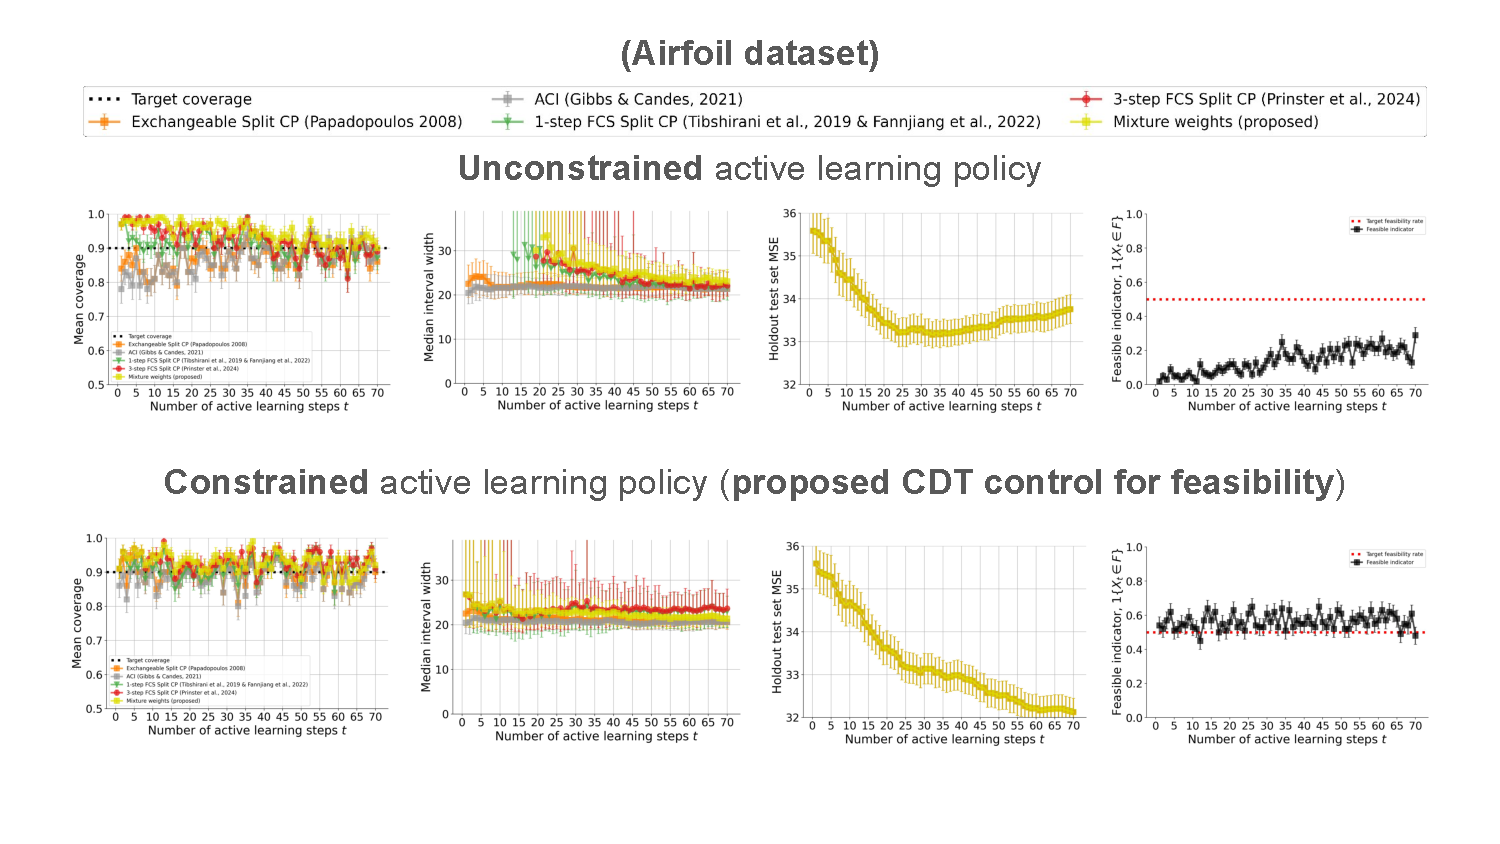
\includegraphics[width=\textwidth]{figures/airfoil.pdf}
    \caption{Results for airfoil UCI dataset.}
\end{figure}

\begin{figure}
    \includegraphics[width=\textwidth]{figures/communities.pdf}
    \caption{Results for communities UCI dataset.}
\end{figure}

\begin{figure}
    \includegraphics[width=\textwidth]{figures/meps.pdf}
    \caption{Results for meps UCI dataset.}
\end{figure}



Experimental details:
\begin{itemize}
    \item \textit{Feasibility labels simulated to decay with 'distance' from source distribution:} Recalling how in our previous paper we simulated selection bias by selecting the training/cal set with probability proportional to $exp(\gamma * X^{pca1})$  where $X^{pca1}$  is the projection of the data onto its 1st principal component, here I sampled feasibility labels from $Bernoulli(p_i)$  where $p_i \propto exp(\gamma * X^{pca1}_i)$ for each point, to simulate the training data being biased toward high feasibility (eg, around 70\%) but the average feasibility across the pool being much lower (eg, around 25\% or so).
    \item \textit{Simplified incumbent policy (for easier implementation here):} Just for simpler implementation at the moment, I just kept the "incumbent policy" as the initial source distribution, meaning that at each t, $\pi_t^{\lambda_t} := \lambda_t * \pi_0 + (1-\lambda_t) * \pi_t^{aggressive}$ , where the difference is using $\pi_0$ in the mixture at the moment rather than $\pi_{t-1}^{\lambda_{t-1}}$.
    \item \textit{Addressing "pin" in theory we'd discussed}: Re discussion about "pin" in theory for how much weight to put on the test point when selecting a risk-controlled policy, I changed from using the "expectation" of the weight to using the maximum weight over the pool set. This is more conservative, and I think almost certainly valid, whereas I think there was an issue with how I was thinking about "expected" weight before (where may need to be a weighted average over the weights, to account for how by construction it's much more common to sample points that the policy gives high weight to).
\end{itemize}





\section{Discussion}

\bibliography{references}
\bibliographystyle{iclr2026_conference}

\appendix
\section{Appendix}
You may include other additional sections here.



\section{Scratch}


Let $\mathcal{X}$ denote the space of possible inputs/contexts/states (e.g., possible protein sequences $\mathbf{x}\in \mathcal{V}^*$, for a vocabulary $\mathcal{V}$), $\mathcal{Y}$ denote the space of a response/outcome variable we care about (e.g., binding affinity or therapeutic efficacy), and let $a:\mathcal{X}\rightarrow \mathcal{X}$ denote the actions that we can take to modify/change/intervene on the space of states/inputs (e.g., modifying some wild-type seed protein sequence $\mathbf{x_0}$ to some designed sequence $\mathbf{x}'$). Furthermore, at each time $t\in [T]$, let $L_t:=L(a(X_t), Y_t)$ denote some loss/cost to taking action $a(X_t)$ and observing $Y_t$ (e.g., in our running protein design example, it may be necessary to ensure that a designed protein sequence is in some set of \textit{feasible} sequences $\mathcal{F}$, and we could use the loss $L_t(X_t')=\mathbbm{1}\{X_t'\not\in\mathcal{F}\}$). Then, our general decision-making goal is the following:
\begin{align*}
    \argmax_{a_t}\quad u(a_t(X_t)) \quad \text{s.t.} \quad L_t \leq \alpha.
\end{align*}

General proxy problem:
\begin{align*}
    \argmax_{a_t}\quad \mathbb{E}[u(a_t(X_t))] \quad \text{s.t.} \quad \mathbb{E}[L_t] \leq \alpha.
\end{align*}

Proxy problem for protein design example: denote design sequence $X_t':=a_t(X_t)$ and loss $L_t:=\mathbbm{1}\{X_t'\not\in\mathcal{F}\}$:
\begin{align*}
    \argmax_{X_t'}\quad \mathbb{E}[u(X_t')] \quad \text{s.t.} \quad & \mathbb{E}[\mathbbm{1}\{X_t'\not\in\mathcal{F}\}] \leq \alpha \\
    & \mathbb{P}(X_t'\not\in\mathcal{F}) \leq \alpha.
\end{align*}


In particular, assume we start with a pre-trained LLM model $\pi_{\theta_0}(\mathbf{x}):\mathcal{X}\rightarrow [0,1]$ denote a pre-trained model (e.g., LLM) with parameters $\theta_0$, which could be written autoregressively as $\pi_{\theta_0}(\mathbf{x})=\prod_{i=1}^{|\mathbf{x}|}\pi_{\theta_0}(x_i\mid x_{<i})$. Now consider prompting $\pi_{\theta_0}$ with some seed sequence $\mathbf{x}_0$ with the goal of finding some design sequence $\mathbf{x}_0'$ that improves the utility function (e.g., binding affinity: $u(\mathbf{x}_0') - u(\mathbf{x}_0)>\epsilon$. For example, might sample with probabilities 
$$p_{\theta_0}(\mathbf{x}_0'|\mathbf{x}_0)\propto \exp(\lambda*(\hat{u}(\mathbf{x}_0') - \hat{u}(\mathbf{x}_0)))$$.

Goal: at each time $t$, propose sequences $X_t'\sim p_{\theta_t}$ s.t. loss is controlled.


% Note that $\pi_{\the`ta_0}$ defines a policy for an initial action, 



the true utility (e.g., binding affinity or therapeutic efficacy) for any sequence $x\in \mathcal{X}$, and $\mathcal{F}\subseteq \mathcal{X}$ the subset of protein sequences that are physically/biologically feasible to produce. The true problem we are interested in is to find a feasible sequence $x'$ that maximizes the utility:
\begin{align}
    x' = \argmax u(x) \quad \text{ s.t. } \quad x \in \mathcal{F}.
\end{align}

In practice, we do not have access to the true utility function $u$, however, so we instead solve a proxy problem. That is, with $\hat{u}:\mathcal{X}\rightarrow \mathbb{R}$ denoting our regression model for the true utility function $u$ and $p(\cdot \mid \hat{u}, D_{1:(t-1)})$ denoting our policy for sampling design sequences (e.g., $p(\cdot \mid \hat{u}, D_{1:(t-1)}) \propto \exp(\lambda \cdot \hat{u})$ for some temperature parameter $\lambda$), in practice we try to solve
\begin{align}
    x_t = \argmax \mathbb{E}[u(x)] \quad \text{ s.t. }\quad \mathbb{P}(x_t \not\in \mathcal{F})\leq \alpha \quad \forall \quad t.
\end{align}





\textbf{Problem formulation:} There are a few aesthetic choices we should make to determine how to frame our problem, which can all yield equivalent formulations, but affect framing:
\begin{itemize}
    \item \textbf{Objective:} Minimizing loss vs maximizing utility
    \item \textbf{Constraint:} Helpful to decide if constraint is on the objective function directly, or if is on a separate cost function. Additionally, different types of constraints:
    \begin{itemize}
        \item \textit{Controlling risk in expectation} (e.g., \citet{angelopoulos2022conformal}): Want expectation of loss to be below some \textit{user-specified, fixed} $\alpha$:
        \begin{align}
            \mathbb{E}[\mathcal{L}(a(X),Y))] \leq \alpha
        \end{align}\label{eq:risk_control}
        \drew{Note: There may not be an action $a$ that satisfies this.}
        \item \textit{Controlling risk in probability} (e.g., contextual bandits): Want probability of the loss exceeding some \textit{fixed} safety-threshold $\tau$ to be no more than some \textit{user-specified, fixed} $\alpha$:
        \begin{align}
            & \mathbb{P}[l(a(X),Y)) > \tau] \leq \alpha \\
            \iff & \mathbb{E}[\mathbbm{1}\{l(a(X),Y)) > \tau\}] \leq \alpha \nonumber \\
            \iff & \eqref{eq:risk_control} \ \text{ if } \ \mathcal{L}(a(X),Y)) = \mathbbm{1}\{l(a(X),Y)) > \tau\} \nonumber 
        \end{align}
        \drew{Note: There may not be an action $a$ that satisfies this.}
        \item \textit{Risk assessment} (e.g., \citet{prinster2022jaws}): \textit{Find minimum upper-bound}, $\alpha_R$, on the probability that an action is unsafe---i.e., exceeds a user-specified, \textit{fixed safety threshold,} $\tau$:
        \begin{align*}
            \alpha_R = \min\big(\big\{\alpha' \ : \ \mathbb{P}[l(a(X),Y)) > \tau] \leq \alpha'\big\}\big)
        \end{align*}
        \item \textit{Optimizing value-at-risk} (e.g., \citet{kiyani2025decision}): Maximize largest value such that, if action $a$ is taken when facing $x$, then utility is at least $\nu(a;x)$ with probability at least some \textit{user-specified, fixed} $1-\alpha$:
        \begin{align*}
            \max_{a, \nu} \quad & \mathbb{E}_{a, \nu}\big[\nu(X)\big] \nonumber \\
            s.t. \quad \& \mathbb{P}\big[u(a(X),Y)\geq \nu(X)\big] \geq 1-\alpha.
        \end{align*}
        Framed in terms of losses rather than utilities (i.e., letting $l=-u$ and $\tau(\cdot)=-\nu(\cdot)$, this is
        \begin{align*}
            \min_{a, \tau} \quad & \mathbb{E}_{a, \tau}\big[\tau(X)\big] \nonumber \\
            s.t. \quad & \mathbb{P}\big[l(a(X),Y)\geq \tau(X)\big] \leq \alpha.
        \end{align*}
    \end{itemize}
\end{itemize}


Let $\mathcal{X}$ denote the space of potential protein sequences, $u(x):\mathcal{X}\rightarrow \mathbb{R}$ denote the true utility (e.g., binding affinity or therapeutic efficacy) for any sequence $x\in \mathcal{X}$, and $\mathcal{F}\subseteq \mathcal{X}$ the subset of protein sequences that are physically/biologically feasible to produce. The true problem we are interested in is to find a feasible sequence $x'$ that maximizes the utility:
\begin{align}
    x' = \argmax u(x) \quad \text{ s.t. } \quad x \in \mathcal{F}.
\end{align}

In practice, we do not have access to the true utility function $u$, however, so we instead solve a proxy problem. That is, with $\hat{u}:\mathcal{X}\rightarrow \mathbb{R}$ denoting our regression model for the true utility function $u$ and $p(\cdot \mid \hat{u}, D_{1:(t-1)})$ denoting our policy for sampling design sequences (e.g., $p(\cdot \mid \hat{u}, D_{1:(t-1)}) \propto \exp(\lambda \cdot \hat{u})$ for some temperature parameter $\lambda$), in practice we try to solve
\begin{align}
    x_t = \argmax \mathbb{E}[u(x)] \quad \text{ s.t. }\quad \mathbb{P}(x_t \not\in \mathcal{F})\leq \alpha \quad \forall \quad t.
\end{align}

\drew{Note: Update notation in proxy problem to be more explicit}

\drew{Question: In practice, is only one designed sequence sent to the lab at a time? Or, are several candidates all sent at the same time?}

Potentially could consider stronger versions of the constraint, i.e., sequential anytime-valid version, which would control the probability of \textit{ever} having a proposed design sequence that's not feasible:
\begin{align}
    \mathbb{P}(\exists \  t : \ x_t \not\in \mathcal{F})\leq \alpha
\end{align}
However, the anytime-valid control is often considered overly conservative, as it controls the probability of a false positive \textit{ever} occuring in an infinite sequence. An intermediately-strong constraint could be instead to control the probability of a false positive among a batch of $T$ designed sequences, i.e., an infeasible sequence at some time $t\in [T]:=\{1, ..., T\}$:
\begin{align}
    \mathbb{P}(\exists \  t \in [T] : \ x_t \not\in \mathcal{F})\leq \alpha
\end{align}



\subsection{Initial draft from Sam}

We train a policy $\pi_\theta(x' \mid x)$ using the FReKL loss on a dataset of matched improving pairs constructed as follows. For each pair of sequences $(x, x')$ within a specified edit distance, we assign rewards:
\begin{equation}
r(x, x') = \begin{cases}
\max(f(x') - f(x), 0) & \text{if } x \in \mathcal{F} \text{ and } x' \in \mathcal{F} \\
1 & \text{if } x \notin \mathcal{F} \text{ and } x' \in \mathcal{F} \\
0 & \text{if } x \notin \mathcal{F} \text{ and } x' \notin \mathcal{F} \\
-1 & \text{if } x \in \mathcal{F} \text{ and } x' \notin \mathcal{F}
\end{cases}
\end{equation}
where $\mathcal{F}$ denotes the feasible set and $f$ is the objective function. This reward structure encourages the policy to maintain feasibility while seeking improvements, with explicit penalties for constraint violations.

To generate queries with controlled risk, we sample a library $\mathcal{L} = \{(x_i, x'_i)\}_{i=1}^N$ from the trained policy and define a nonconformity score $s(x, x') = -\log \pi_\theta(x' \mid x)$.
\textcolor{red}{Consider $-\log \pi_\theta(x' \mid x) - \log \hat p(x)$, where $\hat p(x)$ is our estimate of the prompt distribution.}
We seek a threshold $\lambda$ such that the filtered set
\begin{equation}
\mathcal{C}_\lambda = \{(x, x') \in \mathcal{L} : s(x, x') \leq \lambda\}
\end{equation}
satisfies the risk constraint $\mathbb{E}[\mathbf{1}\{x' \notin \mathcal{F}\}] \leq \alpha$ for a user-specified tolerance $\alpha$.

\drew{Conformal risk control requires that the loss function, in this case $L_i(\lambda):=\mathbbm{1}\{x_j'\not\in\mathcal{F}\}$, is \textit{non-increasing} in $\lambda$. In what's written here, however, increasing $\lambda$ seems like it would \textit{increase} $L_i(\lambda):=\mathbbm{1}\{x_j'\not\in\mathcal{F}\}$; in other words, increasing the size of the filtered set seems like it would \textit{increase} the rate at which the designed sequence is infeasible... It might work, however, if instead use the threshold as $1/\lambda$ in the above.}

Since our calibration data $\mathcal{D}_{\text{cal}} = \{(x_j, x'_j, \mathbf{1}\{x'_j \in \mathcal{F}\})\}_{j=1}^n$ comes from previous rounds of policy execution, we must account for multi-step feedback covariate shift (MFCS). Let $\pi_t$ denote the policy at round $t$ and $P_t$ the induced data distribution. For calibration data from round $t$ evaluated under the current policy $\pi_T$, we compute importance weights:
\begin{equation}
w_j = \frac{p_T(x_j)}{p_t(x_j)} \approx \frac{\pi_T(x_j)}{\pi_t(x_j)}
\end{equation}
The threshold $\lambda$ is then chosen as the smallest value satisfying:
\begin{equation}
\sum_{j=1}^n w_j \mathbf{1}\{s(x_j, x'_j) > \lambda\} \mathbf{1}\{x'_j \notin \mathcal{F}\} + \frac{1}{n_{\text{eff}} + 1} \leq \alpha
\end{equation}
where $n_{\text{eff}} = 1/\sum_{j=1}^n w_j^2$ is the effective sample size.

Given the filtered library $\mathcal{C}_\lambda$, we construct query batches by sampling uniformly at random without replacement, ensuring each selected transition satisfies the calibrated risk bound while maintaining diversity in exploration.

\vspace{2in}



\end{document}
